\documentclass[../../main.tex]{subfiles}
\begin{document}
\begin{oframed}
  \subfile{problem}
\end{oframed}

{\bf [解答]}

\begin{figure}[htb]
  \centering
  % a=1 (e^{1/a}=e) とした y=f(x) の概形と囲まれる面積 S
  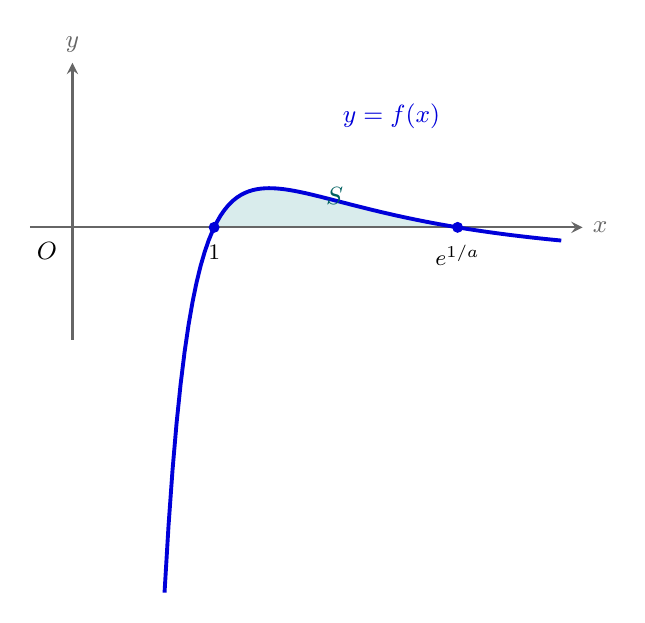
\begin{tikzpicture}[x=1.8cm, y=2.2cm, >=stealth, every node/.style={font=\small}]
    \coordinate (O) at (0,0);
    % 領域 S の淡い塗り
    \fill[teal!15] (1,0) --
    plot[domain=1:2.718, samples=70] (\x, {(2.718/\x - 1)*ln(\x)/\x})
    -- (2.718,0) -- cycle;
    % 座標軸
    \draw[->, thick, gray!80!black] (-0.3,0) -- (3.6,0) node[right] {$x$};
    \draw[->, thick, gray!80!black] (0,-0.65) -- (0,0.95) node[above] {$y$};
    % 曲線 y = f(x)
    \draw[line width=1.4pt, blue!85!black, domain=0.65:3.45, samples=100]
    plot (\x, {(2.718/\x - 1)*ln(\x)/\x});
    % 交点 1, e^{1/a}
    \node[circle, fill=blue!85!black, inner sep=1.4pt] at (1,0) {};
    \node[circle, fill=blue!85!black, inner sep=1.4pt] at (2.718,0) {};
    \node[below=3pt, font=\footnotesize] at (1,0) {$1$};
    \node[below=3pt, font=\footnotesize] at (2.718,0) {$e^{1/a}$};
    \node[below left=2pt] at (O) {$O$};
    % ラベル
    \node[teal!75!black, font=\small] at (1.85,0.18) {$S$};
    \node[above right=2pt, blue!85!black] at (1.8,0.48) {$y=f(x)$};
  \end{tikzpicture}
  \caption{$y=f(x)$のグラフと$x$軸で囲まれる領域$S$（$1\le x\le e^{1/a}$）}
  \label{fig:fx_area_s}
\end{figure}

与えられた関数
\begin{align}
  f(x)=\left(\dfrac{e}{x^a}-1\right)\dfrac{\log x}{x} \quad (a,x > 0) \label{eq:1}
\end{align}
について考える．
$f(x)\geqq0$となるのは$1\leqq x\leqq e^{1/a}$の時だから，
求める面積を$S$とすると
\begin{align}
  S
  & =\int_1^{e^{1/a}}f(x)\,dx  \\
  & =\int_1^{e^{1/a}}\left(\dfrac{e}{x^a}-1\right)\dfrac{\log x}{x} \,dx  \label{eq:2}
\end{align}
である．
各項個別に計算すると
\begin{align}
  (\text{第1項})
  &=\int_1^{e^{1/a}}\dfrac{\log x}{x^{a+1}}\,dx \\
  &=\left[-\dfrac{1}{a}\dfrac{\log x}{x^a}\right]_1^{e^{1/a}}
  +\int_1^{e^{1/a}}\dfrac{1}{a x^{a+1}}\,dx\\
  &=\left[-\dfrac{1}{a}\dfrac{\log x}{x^a}-\dfrac{1}{a^2 x^a}\right]_1^{e^{1/a}}\\
  &=-\dfrac{1}{a^2 e}-\dfrac{1}{a^2 e}+\dfrac{1}{a^2} \\
  &=\dfrac{1}{a^2}\left(1-\dfrac{2}{e}\right) \\
  (\text{第2項})
  &=\int_1^{e^{1/a}}\dfrac{\log x}{x}\,dx \\
  &=\left[\dfrac{1}{2}(\log x)^2\right]_1^{e^{1/a}} \\
  &=\dfrac{1}{2a^2}
\end{align}
だから，\cref{eq:2}に代入して求める面積は
\begin{align}
  S
  =\dfrac{e}{a^2}\left(1-\dfrac{2}{e}\right)-\dfrac{1}{2a^2}
  =\dfrac{1}{a^2}\left(e-\dfrac{5}{2}\right)
\end{align}
である．

\end{document}
